\documentclass[conference]{IEEEtran}
% \IEEEoverridecommandlockouts

\usepackage{cite}
\usepackage{amsmath,amssymb,amsfonts}
\usepackage{algorithmic}
\usepackage{graphicx}
\usepackage{subcaption}
\usepackage{textcomp}
\usepackage{amsmath}
\usepackage{url}
\usepackage{booktabs}
\usepackage[dvipsnames]{xcolor}
\def\BibTeX{{\rm B\kern-.05em{\sc i\kern-.025em b}\kern-.08em
    T\kern-.1667em\lower.7ex\hbox{E}\kern-.125emX}}
\begin{document}

\title{Mechanistic Isolation and Causal Verification of Induction Circuits in GPT-2 Small\\ }

\author{\IEEEauthorblockN{Kritika Pandit}
\IEEEauthorblockA{\textit{Independent Research} \\ % TODO: update affiliation
Northfield, Minnesota \\ % TODO: update location if needed
panditk@carleton.edu}
}

\maketitle

\begin{abstract}

The standard mechanistic interpretability narrative posits that transformer language models perform in-context pattern replication of the form \texttt{... A B ... A -> B} via specialized ``induction heads.'' This narrative was originally formalized by Olsson et al. (2022). Observational metrics such as attention pattern matching strongly suggest the existence of these heads, but observational correlation alone cannot establish whether a given head's output is causally responsible for downstream logit shifts, whether that responsibility is concentrated in monosemantic sub-head features rather than smeared across the whole head, or whether the circuit can be recovered without hand-picking candidates from those same observational scores. This paper investigates the induction mechanism in GPT-2 small across six linked experiments: (1) correlational localization of candidate heads via attention-pattern scoring, (2) causal confirmation via activation patching, (3) stress-testing the inferred mechanism against a positional-heuristic confound and a cross-distribution equifinality test, (4) causal verification of upstream $K$-composition with a previous-token head, (5) feature-level decomposition of the causal signal using sparse autoencoders, and (6) automated, hypothesis-free circuit discovery via attribution patching. We find that induction in GPT-2 small is a distributed five-head circuit (80.3\% joint logit recovery) rather than a single dominant head (5.5--7.9\% each), that this circuit causally depends on a specific upstream previous-token head (a 0.240 attention-score drop under ablation versus $-0.003$ for a control), that the causal signal inside each head is not concentrated in a small number of sparse-autoencoder features (under 1.5\% recovery from the top 10 of $\sim$49k), and that automated gradient-based discovery recovers 4 of 5 hand-picked heads in a single backward pass but underranks the single most attention-salient head due to a known saturated-softmax failure mode (Spearman $\rho = 0.44$ against ground-truth patching). Two experimental design flaws were identified and corrected in the course of this work; both are reported alongside the corrected results.

\end{abstract}

\section{Introduction}

Mechanistic interpretability aims to reverse-engineer the algorithms a neural network has learned, rather than treating it as a black box characterized only by its input-output behavior. A recurring finding in this literature is the \emph{induction head}: an attention head that, given a sequence of the form \texttt{... A B ... A}, attends from the second occurrence of token $A$ back to the token $B$ that followed its first occurrence, and copies information consistent with predicting $B$ next~\cite{olsson2022}. Because this behavior generalizes to sequences of tokens the model has never seen during training, it is widely cited as direct mechanistic evidence for in-context learning.

However, most treatments of induction heads stop at the observational level. This is true even of standard interpretability tutorials. A head is identified as an ``induction head'' simply because its attention pattern matches the expected shape on synthetic repeated sequences. This leaves several questions unresolved. First, does a high observational score imply that the head's output is causally responsible for the model's downstream prediction, or could the correlation be incidental to a computation carried out elsewhere? Second, if a head's output is causally responsible, is the relevant information concentrated in the head as a whole, or could it be further decomposed into a small number of interpretable sub-head features, consistent with the superposition hypothesis~\cite{bricken2023}? Third, can the circuit be recovered by an automated, hypothesis-free method, or does its discovery fundamentally depend on the researcher hand-picking candidates from an observational score in the first place?

This paper addresses these questions directly, using GPT-2 small as a test model and TransformerLens as the analysis framework. We organize the investigation around six linked experiments:

\begin{enumerate}
    \item \textbf{Correlational localization}: identify candidate induction heads via an attention-based induction score on synthetic repeated sequences.
    \item \textbf{Causal activation patching}: determine whether the identified heads' outputs are individually and jointly necessary and sufficient to recover the correct next-token logit.
    \item \textbf{Stress-testing}: attempt to falsify the inferred mechanism via an exact-match corruption test and a cross-distribution stability test, explicitly reporting an experimental design flaw uncovered in the process.
    \item \textbf{Upstream $K$-composition verification}: test whether the induction heads causally depend on a specific upstream previous-token head, again reporting and correcting an initial flawed test design.
    \item \textbf{Feature-level decomposition}: use sparse autoencoders trained on head outputs to test whether the causal signal is concentrated in a small number of monosemantic features.
    \item \textbf{Automated circuit discovery}: test whether attribution patching, a gradient-based linear approximation to activation patching, can recover the same circuit without hand-picked candidates.
\end{enumerate}

The remainder of this paper is organized as follows. Section~II reviews related work in transformer circuit analysis, sparse autoencoders, and automated circuit discovery. Section~III describes the experimental methodology for each of the six experiments. Section~IV presents the results. Section~V discusses the implications, limitations, and concludes.

\section{Literature Review}

The theoretical foundation for this work is the transformer circuits framework of Elhage et al.~\cite{elhage2021}, which formalizes attention heads as composed of an independent query-key (QK) circuit, determining \emph{where} a head attends, and an output-value (OV) circuit, determining \emph{what} it writes once attending there. This framework introduces the notion of $K$-composition, in which one head's output is read by a later head's key computation, and identifies induction heads as a canonical example of an algorithm that requires two-layer composition and cannot be implemented by a single attention layer.

Olsson et al.~\cite{olsson2022} provide the primary empirical characterization of induction heads, arguing that they are a broadly universal circuit across model scales and that their formation coincides with a phase transition in the loss curve associated with the onset of in-context learning. This paper's Experiment~1 and~2 directly test the localization and causal-sufficiency claims that motivate this narrative in the specific case of GPT-2 small.

Prior work has used activation patching to identify circuits responsible for specific narrow behaviors in GPT-2 small; most notably, Wang et al.~\cite{wang2022} isolate the circuit responsible for indirect object identification, establishing the general methodology of comparing clean and corrupted prompt pairs and patching intermediate activations to localize causally relevant components. The present paper applies the same causal-intervention logic to induction, but additionally probes upstream composition (Experiment~4) and automated recoverability (Experiment~6), which are not addressed in that line of work.

Variengien~\cite{variengien2023} raises a direct methodological caution relevant to this paper's motivation: that the induction-head hypothesis is frequently treated by the community as a cleaner, more monolithic algorithmic story than the underlying evidence actually supports. This paper's Section~III-D (the exact-match robustness test) and Section~III-C (the corrected path-patching test) are direct, if partial, responses to this caution. Both sections report an initial test that appeared to support a clean textbook claim. Both are followed by identification of a confound or design flaw that complicates that interpretation.

The premise that individual head or neuron activations may not be the correct unit of analysis is developed in the superposition literature. Bricken et al.~\cite{bricken2023} demonstrate that sparse autoencoders (SAEs) trained to reconstruct a model's internal activations with an L1 sparsity penalty can recover interpretable, approximately monosemantic feature directions from otherwise polysemantic activation space. Kissane et al.~\cite{kissane2024} extend this specifically to attention layer outputs (\texttt{hook\_z}), showing that SAEs trained on this site are practically useful for attributing behavior to specific heads and features. This paper's Experiment~5 directly builds on that methodology, using SAELens~\cite{bloom2024} to train and query such SAEs on the induction heads identified in Experiment~1.

Finally, this paper's Experiment~6 draws on the attribution patching literature. Nanda~\cite{nanda2023attrpatch} proposes attribution patching as a gradient-based linear approximation to activation patching that reduces the cost of scoring all components in a network from one forward pass per component to a single forward-and-backward pass. Syed et al.~\cite{syed2023} formalize an edge-level variant of this approach and show it can outperform slower search-based automated circuit discovery methods such as ACDC~\cite{conmy2023} in practice, while noting known failure modes around saturated nonlinearities. This paper's Experiment~6 empirically reproduces one such failure mode in the specific context of the induction circuit identified in Experiments~1--4.

\section{Methodology}
\label{sec:method}

\subsection{Model and General Experimental Framework}

All experiments use GPT-2 small (12 layers, 12 heads per layer, 768-dimensional residual stream), accessed via the TransformerLens library, which exposes every intermediate activation as a named hook point that can be read or overwritten during a forward pass. Experiments~1--4 use a common synthetic sequence paradigm: a \emph{clean} sequence of the form \texttt{[BOS, A, A]}, where $A$ is a sequence of independently sampled random token IDs, and, where a causal comparison is required, a \emph{corrupted} sequence \texttt{[BOS, A, B]}, where $B$ is an independently sampled sequence of the same length. Because $A$ is drawn uniformly at random, correctly predicting the continuation of the second copy of $A$ cannot be explained by memorized pretraining statistics and must reflect an in-context copying mechanism.

\subsection{Experiment 1: Correlational Localization}

For every attention head in every layer, we define the \emph{induction score} as the average attention weight, over a batch of clean sequences, allocated from a destination position in the second copy of $A$ back to the source position immediately following that token's first occurrence. This score is computed via a forward-pass hook attached to each layer's attention pattern tensor, requiring a single forward pass over the full $12\times12$ head grid.

\subsection{Experiment 2: Causal Activation Patching}

To test whether a high induction score corresponds to causal importance, we run the model on the corrupted sequence while overwriting one or more heads' \texttt{hook\_z} output (the per-head output prior to the output projection $W_O$) with the value taken during a clean run, holding all other activations at their corrupted values. We measure the percentage of the clean-versus-corrupted logit gap on the correct continuation token that is recovered by this intervention, for individual heads, cumulative subsets of heads, and, as a validity sanity check, the entire residual stream at a given layer.

\subsection{Experiment 3: Stress-Testing the Inferred Mechanism}

\subsubsection{Exact-match corruption test}
The textbook definition of an induction head requires attention based on exact token identity, not merely a fixed positional offset. To test this, a single token in the second copy of $A$ is replaced with a different random token, and the induction score at exactly that position is compared against the average score at all unaffected positions. If the head performs true content matching, its attention at the corrupted position should collapse toward baseline.

\subsubsection{Cross-distribution stability test}
To test whether the same heads handle induction regardless of input content, or whether a different subset of heads is recruited for different content types (an instance of \emph{equifinality}), the induction score computation from Experiment~1 is repeated on three distinct data distributions: uniformly random tokens, a natural-language paragraph repeated as its own continuation, and a repeated sequence of single-digit numeric tokens. The top-5 scoring heads are compared for set overlap across distributions.

\subsection{Experiment 4: Upstream $K$-Composition Verification}

\subsubsection{Previous-token head identification}
Analogous to the induction score, a \emph{previous-token score} is computed as the average attention paid from each position to the immediately preceding position, on ordinary (non-repeated) context, to identify the head responsible for writing local positional information into the residual stream.

\subsubsection{Path-patching attempt}
An initial test patched the identified previous-token head's \texttt{hook\_z} output from a clean run into a corrupted run, and measured the resulting change in a receiver induction head's attention pattern. As reported in Section~IV-D, this test produced a null result attributable to a design flaw: because the corrupted sequence alters the token identity at the receiver's own query position, no upstream patch can repair a query built from the wrong token identity, since $K$-composition governs the key side of the computation, not the query side.

\subsubsection{Corrected ablation test}
To isolate the $K$-composition dependency without corrupting the query token identity, the corrected test remains entirely within the clean run and instead mean-ablates the candidate previous-token head's output (replacing its activation at each position with the batch mean at that position), comparing the resulting change in the receiver head's induction score against ablation of a control head with the lowest previous-token score.

\subsection{Experiment 5: Feature-Level Decomposition via Sparse Autoencoders}

Because a head's 64-dimensional \texttt{hook\_z} output could itself encode multiple unrelated computations in superposition~\cite{bricken2023}, sparse autoencoders trained on GPT-2 small's \texttt{hook\_z} activations~\cite{kissane2024}, obtained via SAELens~\cite{bloom2024}, are used to test whether the causal signal identified in Experiment~2 is concentrated in a small number of monosemantic feature directions. Two quantities are computed for each of the four induction heads with confirmed causal contribution: (i) a \emph{full SAE reconstruction} recovery, in which the head's clean activation is replaced by the SAE's decode-of-encode using its entire feature dictionary (establishing a ceiling on what the dictionary can represent at all, independent of feature selection), and (ii) a \emph{head-restricted feature} recovery, in which only the single feature (or top 10 features) most attributable to that head by decoder-weight norm and most active at the induction-relevant positions is used for reconstruction.

\subsection{Experiment 6: Automated Circuit Discovery via Attribution Patching}

To test whether the circuit identified by hand in Experiments~1--4 can be recovered without a hand-picked observational starting point, we apply attribution patching~\cite{nanda2023attrpatch}, a first-order Taylor approximation to activation patching:
$$
\text{predicted\_effect(head)} \approx \nabla_{z}\,\text{metric}\big|_{z_{\text{corrupted}}} \cdot \big(z_{\text{clean}} - z_{\text{corrupted}}\big),
$$
which ranks all 144 heads in the network using a single corrupted forward-and-backward pass plus one clean forward pass, in contrast to the one-forward-pass-per-head cost of the exhaustive procedure used by hand in Experiment~2. The resulting top-10 ranked heads are cross-validated against ground-truth activation patching, and the Spearman rank correlation between predicted attribution magnitude and measured recovery is reported.

\section{Results}
\label{sec:results}

\subsection{Correlational Localization}

Table~\ref{tab:induction_scores} reports the induction scores for the top five candidate heads and a negative control. The score distribution is sparse, with high scores concentrated in layers 5 through 7 rather than diffusely spread across the network, and the top-scoring heads match those reported in the foundational literature~\cite{olsson2022}, providing an external check that the pipeline is not recovering a setup-specific artifact. Figure~\ref{fig:heatmap} shows the full $12\times12$ induction score matrix.

\begin{table}[htbp]
\centering
\caption{Induction Scores for Top Candidate Heads}
\label{tab:induction_scores}
\begin{tabular}{lcl}
\toprule
\textbf{Layer \& Head} & \textbf{Induction Score} & \textbf{Functional Designation} \\
\midrule
L5H5  & 0.926 & Candidate Induction Head \\
L6H9  & 0.921 & Candidate Induction Head \\
L7H10 & 0.914 & Candidate Induction Head \\
L5H1  & 0.903 & Candidate Induction Head \\
L7H2  & 0.822 & Candidate Induction Head \\
L4H11 & 0.000 & Negative Control Head \\
\bottomrule
\end{tabular}
\end{table}

\begin{figure}[htbp]
    \centering
    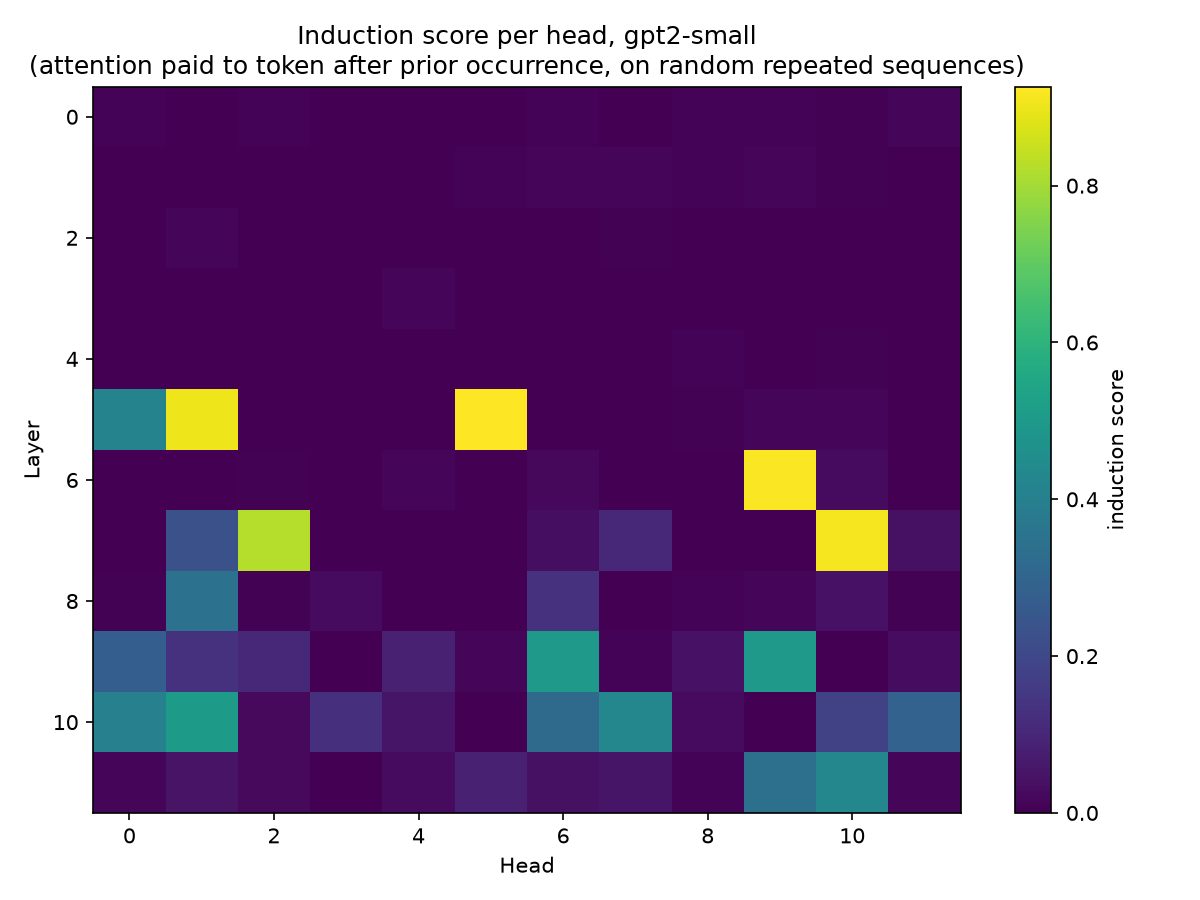
\includegraphics[width=0.9\linewidth]{images/induction_score_heatmap.png}
    \caption{Induction score across all 144 heads of GPT-2 small. Scores are sharply localized in layers 5--7 rather than diffusely distributed.}
    \label{fig:heatmap}
\end{figure}

\subsection{Causal Activation Patching}

Table~\ref{tab:patching} reports logit recovery under activation patching. No individual head recovers more than 8\% of the clean-versus-corrupted logit gap, despite each scoring above 0.82 observationally. Recovery increases from 31.8\% (top 3 heads) to 80.3\% (top 5 heads) as heads are added cumulatively, indicating a distributed circuit rather than a single dominant head. The control head recovers 0.1\%, and the full-residual-stream sanity check recovers 100.0\%, confirming both the specificity and the validity of the patching procedure.

\begin{table}[htbp]
\centering
\caption{Activation Patching: Logit Recovery}
\label{tab:patching}
\begin{tabular}{lc}
\toprule
\textbf{Intervened Activation (\texttt{hook\_z})} & \textbf{Logit Recovery} \\
\midrule
L5H5 alone & 5.8\% \\
L6H9 alone & 7.9\% \\
L7H10 alone & 5.5\% \\
L4H11 alone (control) & 0.1\% \\
L5H5 + L6H9 + L7H10 & 31.8\% \\
Top 5 heads combined & 80.3\% \\
Full residual stream (post-layer 7) & 100.0\% \\
\bottomrule
\end{tabular}
\end{table}

\subsection{Stress-Testing Results}

\subsubsection{Exact-match corruption test}
Contrary to the naive expectation, the induction score at the corrupted position remained near-ceiling (0.93--0.95), statistically indistinguishable from unaffected positions. Inspection of the experimental design identified the cause: all sequences in the batch shared a fixed period (\texttt{seq\_len=50}), so a head attending to a fixed positional offset would score identically to a genuine content-matching head under this test. The test as designed cannot separate the two hypotheses; this is reported as a corrected limitation rather than a substantive finding about the model (Section~V-C).

\subsubsection{Cross-distribution stability}
The identical set of five heads (L5H5, L6H9, L7H10, L5H1, L7H2) ranked in the top five across all three tested distributions, ruling out equifinality at the level of which heads are recruited. However, the magnitude of the top score varied substantially: 0.94 on random tokens, 0.86 on natural language, and 0.57 on digit sequences, consistent with other predictive pathways (n-gram statistics, syntax) sharing the predictive burden on more structured content.

\subsection{Upstream $K$-Composition Verification}

The previous-token score identified L4H11 as the dominant previous-token head (score 0.985). Notably, this is the same head that scored zero on the induction metric in Experiment~1. The initial path-patching test (patching L4H11's clean output into the corrupted run) yielded 0.1\% recovery of the receiver head's induction score, indistinguishable from a random control, and was diagnosed as invalid due to simultaneous corruption of the receiver's query token identity (Section~III-D.2). The corrected mean-ablation test, reported in Table~\ref{tab:ablation}, shows a substantial and specific effect: ablating L4H11 drops the induction score of receiver head L5H5 by 0.240, while ablating a control head changes it by only $+0.003$.

\begin{table}[htbp]
\centering
\caption{Corrected Ablation Test for $K$-Composition}
\label{tab:ablation}
\begin{tabular}{lccl}
\toprule
\textbf{Condition} & \textbf{L5H5 Score} & \textbf{$\Delta$} & \textbf{Implication} \\
\midrule
Clean baseline & 0.929 & --- & Unperturbed \\
L4H11 ablated & 0.689 & $-0.240$ & Loss of $K$-input \\
L0H5 ablated (control) & 0.932 & $+0.003$ & No impact \\
\bottomrule
\end{tabular}
\end{table}

L5H5 retains an induction score of 0.689 after L4H11 is fully ablated, suggesting partial functional redundancy from other, unidentified previous-token heads.

\subsection{Feature-Level Decomposition}

Table~\ref{tab:sae} reports SAE-based decomposition results for the four induction heads with confirmed causal contribution. Full-dictionary SAE reconstruction recovers 3.5--5.0\% logit recovery, roughly 50--80\% of each head's raw activation-patching recovery from Experiment~2, indicating the relevant direction is largely representable by the trained dictionary. However, the single most head-attributable, most-active feature recovers under 0.2\% in every case, and even the top 10 such features together recover under 1.5\%. Reconstruction error at the induction-relevant positions (54--69\% of activation norm) is substantially elevated relative to the SAE's typical in-distribution performance (10--20\%), since the SAE was trained on natural-language pretraining data rather than the synthetic random-token sequences used here.

\begin{table}[htbp]
\centering
\caption{SAE Feature-Level Decomposition}
\label{tab:sae}
\small
\begin{tabular}{lcccc}
\toprule
\textbf{Head} & \textbf{Head} & \textbf{Full SAE} & \textbf{Best} & \textbf{Top-10} \\
 & \textbf{Recovery} & \textbf{Ceiling} & \textbf{Feature} & \textbf{Features} \\
\midrule
L5H5  & 5.8\% & 4.3\% & 0.0\% & 0.1\% \\
L6H9  & 7.9\% & 5.0\% & 0.2\% & 0.8\% \\
L7H10 & 5.5\% & 3.5\% & 0.1\% & 0.3\% \\
L7H2  & 8.3\% & 4.2\% & 0.1\% & 1.1\% \\
\bottomrule
\end{tabular}
\end{table}

\subsection{Automated Circuit Discovery}

Attribution patching, computed in a single backward pass, ranks 4 of the 5 hand-picked circuit heads (L5H1, L6H9, L7H2, L7H10) within its top 10 of 144 heads. The fifth head, L5H5, was the single highest-scoring head observationally in Experiment~1. It ranks 13th despite its confirmed causal contribution in Experiment~2. This is consistent with the documented failure mode in which a head whose effect passes through a near-saturated softmax attention pattern has a small local gradient relative to its true causal effect. Validating the predicted top-10 heads against real activation patching yields a Spearman rank correlation of $\rho = 0.44$. The automated ranking additionally surfaces four smaller contributors not tested by hand (L9H9, L9H6, L10H0, L10H1; each recovering 3.5--6.1\% on real patching) and two heads with negative attribution (L10H7, L11H10) subsequently confirmed by real patching to actively suppress the correct-token logit, consistent with the copy-suppression phenomenon documented elsewhere in GPT-2 small. The negative control head (L4H11) correctly scores near-zero on both attribution and real patching.

\section{Discussion and Conclusion}

\subsection{Interpreting the Results}

Taken together, these six experiments show a clear separation between what an observational metric can and cannot establish. Attention-pattern induction scores correctly localize the relevant layers (Section~IV-A), but overstate the causal importance of any single head, which is in fact distributed across a five-head circuit (Section~IV-B). This circuit is not an isolated single-layer phenomenon: it causally depends on a specific upstream previous-token head via $K$-composition (Section~IV-D), consistent with the two-layer algorithmic requirement described by Elhage et al.~\cite{elhage2021}. At a finer grain, the causal signal inside each head is not further concentrated into a handful of monosemantic sparse-autoencoder features (Section~IV-E); it is either genuinely smeared across many features, or encoded in a manner this particular SAE does not cleanly capture. The latter explanation is more likely given the elevated reconstruction error. The SAE was trained off-distribution relative to the synthetic random-token sequences used here, which plausibly accounts for that error. Finally, automated discovery is a useful but imperfect substitute for hand-picked, observationally-motivated candidates: it recovers most of the known circuit in a fraction of the compute, but systematically underweights at least one confirmed causal contributor due to a known linearization failure mode (Section~IV-F).

Two points in this investigation are worth highlighting methodologically rather than just empirically. The exact-match corruption test in Section~IV-C.1 initially appeared to refute content-based matching, but the refutation itself was an artifact of a confounded experimental design (constant sequence period). Likewise, the first path-patching attempt in Section~IV-D initially appeared to refute $K$-composition entirely, but was invalidated by a query-side confound rather than reflecting an absence of dependence. In both cases, taking the first result at face value would have produced an incorrect conclusion about the model; identifying and correcting the underlying design flaw, rather than reporting the uncorrected result, was necessary to reach a valid conclusion.

\subsection{Implications}

These results suggest that circuit-analysis claims resting solely on attention-pattern correlation should be treated as a starting hypothesis rather than a conclusion. This holds even when the correlational signal is sparse, well-localized, and consistent with prior literature, as it is here. This has direct relevance for scaling interpretability research: as models grow, exhaustive hand-patching of every component becomes intractable, motivating a workflow in which fast, approximate methods such as attribution patching (Section~IV-F) are used to generate candidate lists, with true activation patching reserved for confirming causal importance among the smaller candidate set. Similarly, sparse-autoencoder-based decomposition is only as reliable as the distributional match between the SAE's training data and the activations under study; the elevated reconstruction error observed here (Section~IV-E) is a caution against over-interpreting negative feature-level results without first checking for this mismatch.

\subsection{Limitations}

Several limitations qualify these findings. First, quantitative recovery metrics were computed from single random seed generations; multi-seed aggregation would establish stability against token-sampling variance. Second, activation swapping was restricted to post-attention head projections (\texttt{hook\_z}); finer-grained patching directly between $W_V$ and $W_K$ projections would more precisely isolate internal tensor pathways. Third, the exact-match corruption test (Section~IV-C.1) requires variable sequence periods per example to properly separate positional-offset heuristics from true content matching; the current fixed-period design cannot distinguish the two. Fourth, the approximately 19.7\% logit-recovery gap between the top-5-head patch and the full-residual-stream sanity check (Table~\ref{tab:patching}) was not localized to specific downstream components. Fifth, the sparse autoencoders used in Section~IV-E were trained on natural-language data rather than the synthetic distribution studied here, which may partly explain the elevated reconstruction error independent of any intrinsic property of the induction computation. Sixth, the automated discovery in Section~IV-F operates at the level of individual nodes (\texttt{hook\_z} sites) rather than sender-receiver edges, and therefore does not by itself recover the $K$-composition dependency established by hand in Section~IV-D; a full edge-level attribution graph~\cite{conmy2023} is the natural extension.

\subsection{Conclusion}

This paper investigated the induction circuit in GPT-2 small across six linked experiments spanning correlational localization, causal activation patching, adversarial stress-testing, upstream composition verification, feature-level decomposition, and automated discovery. The central finding is that induction in GPT-2 small is not a single dominant head but a distributed, five-head circuit with a causally verified upstream dependency, whose signal resists further concentration into a small number of sparse-autoencoder features and is only partially recoverable by fast automated methods. Two experimental design flaws were identified and corrected in the course of this investigation, underscoring that observational and even naively-causal results require active attempts at falsification before being taken as evidence about the underlying model. Future work should extend the automated discovery in Section~IV-F to edge-level attribution graphs to recover the composition structure established by hand in Section~IV-D, and repeat the sparse-autoencoder analysis in Section~IV-E with dictionaries trained on the synthetic distribution studied here.

\begin{thebibliography}{00}

\bibitem{olsson2022}
C. Olsson, N. Elhage, N. Nanda, \textit{et al.}, ``In-context learning and induction heads,'' \textit{Transformer Circuits Thread}, 2022. [Online]. Available: https://transformer-circuits.pub/2022/in-context-learning-and-induction-heads/index.html

\bibitem{elhage2021}
N. Elhage, N. Nanda, C. Olsson, \textit{et al.}, ``A mathematical framework for transformer circuits,'' \textit{Transformer Circuits Thread}, 2021. [Online]. Available: https://transformer-circuits.pub/2021/framework/index.html

\bibitem{wang2022}
K. Wang, A. Variengien, A. Conmy, B. Shlegeris, and J. Steinhardt, ``Interpretability in the wild: a circuit for indirect object identification in GPT-2 small,'' \textit{arXiv:2211.00593}, 2022.

\bibitem{variengien2023}
A. Variengien, ``Some common confusion about induction heads,'' \textit{LessWrong}, 2023. [Online]. Available: https://www.lesswrong.com/posts/nJqftacoQGKurJ6fv/some-common-confusion-about-induction-heads

\bibitem{bricken2023}
T. Bricken \textit{et al.}, ``Towards monosemanticity: decomposing language models with dictionary learning,'' \textit{Transformer Circuits Thread}, 2023. [Online]. Available: https://transformer-circuits.pub/2023/monosemantic-features/index.html

\bibitem{kissane2024}
C. Kissane, R. Krzyzanowski, \textit{et al.}, ``Interpreting attention layer outputs with sparse autoencoders,'' \textit{arXiv:2406.17759}, 2024.

\bibitem{bloom2024}
J. Bloom, ``Open source sparse autoencoders for all residual stream layers of GPT2-small,'' \textit{SAELens / LessWrong}, 2024. [Online]. Available: https://www.lesswrong.com/posts/f9EgfLSurAiqRJySD

\bibitem{nanda2023attrpatch}
N. Nanda, ``Attribution patching: activation patching at industrial scale,'' 2023. [Online]. Available: https://www.neelnanda.io/mechanistic-interpretability/attribution-patching

\bibitem{syed2023}
A. Syed, C. Rager, and A. Conmy, ``Attribution patching outperforms automated circuit discovery,'' \textit{arXiv:2310.10348}, 2023.

\bibitem{conmy2023}
A. Conmy, A. Mavor-Parker, A. Lynch, S. Heimersheim, and A. Garriga-Alonso, ``Towards automated circuit discovery for mechanistic interpretability,'' \textit{arXiv:2304.14997}, 2023.

\end{thebibliography}

\section{Code Availability}
\url{https://github.com/panditk455/Circuit-Causal-Verification}

\end{document}
